\chapter{Dark Matter - The Unknown Mass}

\par
For thousands of years the humans have tried to understand the Universe that we inhabit.
The majestic beauty of the sky has been one of most intriguing things - with our knowledge developing from believing we are the centre to realising that we are a tiny part of the Universe and the Universe is a dynamic and ever changing landscape (all-be-it very slowly on our time-scale).

\par
However, as our understanding increasing, we have realised that we may in-fact understand significantly less of the Universe and it's components that we thought.

What's more amazing is that technological improvements have allowed for a much greater understanding of the Universe we live in.
This has included the first image of a black hole, and the observations of gravitation waves from merging neutron stars. 
TODO add cites.
Though our understanding of what is truly the makeup of our Universe is tiny - at 5\%. 
This leaves a massive amount of unknown.

For nearly a century, cosmological observations have given results that do not fit within the standard model of particle physics (SM), which though can predict most experimental results, cannot account for gravity and conflicts with general relativity. 
This leads for the need to go beyond the SM. It is known that the SM can only account for 5\% of the energy and matter in the Universe. 
The other parts, known as dark matter (DM) and dark energy due to their non-luminous properties are taken into account in the $\Lambda$-CDM model of the Universe which is the most inline with cosmological observations.
It is also interesting to note that extensions to the SM to solve problems such as the hierarchy problem naturally lead to DM.


\par
As technology has advanced we have gained the ability to peer deeper and deeper into space.

\par
In this chapter we summarise the evidence for this unexplained part of our universe.
This is followed by a selection of candidates that have been hypothesised to be dark matter, and the way in which they are being searched for.

\section{The Problem}

\par
As early as 1783, invisible structures in the universe has been hypothesised, but it wasn't until the end of the 19th century, when astronomical photography was realised that observations gave a hint of an invisible mass \cite{History_Of_Dark_Matter_2018_ref}.
These have grown from humble beginnings as a puzzling curiosity that could perhaps be explained away by observational uncertainties to a direct challenge to fundamental particle physics, cosmology and astrophysics.
In this section 

%Some other quotes like
%\par
%Perhaps the most fitting conclusion to this was by Lord Kelvin who concluded
%
%\begin{quote}
%    many of our stars, perhaps a great majority of them, may be dark bodies
%\end{quote}
%
% Add Quote about black holes 17XX :P 


\subsection{Galactic Scale}

\par
Some of the earliest indications of dark matter comes from comparing methods used to estimate the mass of astronomical bodies.
Once such example of this comes from Zwicky, who in 1933 who sought to determine the mass of the Coma Cluster by relating the potential energy to the kinetic energy using the Virial theorem \cite{Fritz_Zwicky_1933_ref}.
Zwicky found that in order to achieve the average observed velocity of 1000 km/s, there would need to be in excess of $\backsim$12 times more mass than estimated using the galaxy radius and 400 times the mass estimated from luminous matter.
This lead him to the conclusion that:
\begin{quote}
``If this should be verified, it would lead to the surprising result that dark matter
exists in much greater density than luminous matter."
\end{quote}
which, although not the first time the use the phrase ``dark matter", is perhaps the most well known instance.
Other studies around the same time came to similar conclusions \cite{hubble_and_co_viral_theorem_ref}.
More modern techniques have found issues with these calculations but the most significant finding of missing mass remains \cite{a_second_history_of_dark_matter_ref}.

\par
Shortly after, in 1941, it was shown that galactic rotation curves could be used as a reliable way of determining the mass distribution within a galaxy \cite{Chandrasekhar_1941_ref}.
From standard Newtonian dynamics, an object in circular motion with mass $m$ has rotation velocity $v$ that follows;
\begin{equation}
    v(r) = \sqrt{\frac{rF}{m}} = \sqrt{\frac{GM(r)}{r}}
    \label{eq:Kepler_Motion}
\end{equation}
where $G$ is the gravitational constant and $M(r)$ is the mass contained within the radius $r$ given by; $M(r) = 4 \pi \int \rho(r) r^{2} dr$.
In a spiral galaxy, the luminous mass is distributed as approximately a disc. 
Using this, we expect the tangential velocity of an object within the galaxy to increase with the radius until the there is equal mass pulling in and out.
After this point the velocity of the object should decrease as $\sqrt{\frac{1}{r}}$ as it becomes further away from the majority of the mass.
However, observations have shown that this is in fact not the case, and instead the velocity distribution remains flat as illustrated in \autoref{fig:DM_Evidence_NGC_6503}.
\begin{figure}[!htbp]%
    \centering
    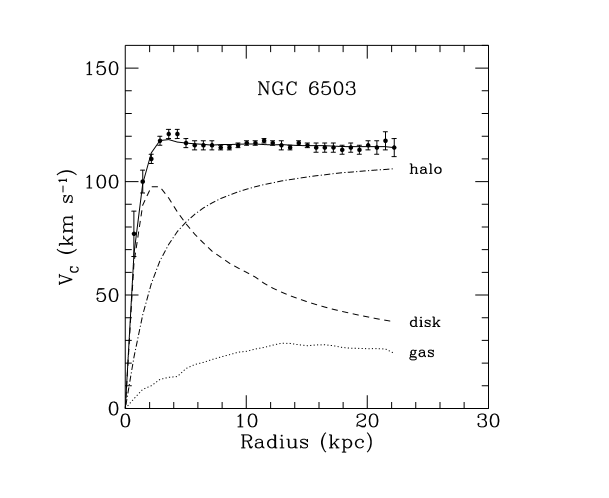
\includegraphics[scale=1.0]{Figures/DarkMatterEvidence/NGC_6503_galaxy_speed.png}
    \caption[Galaxy rotation curve for the NGC 6503 galaxy]{Galaxy rotation curve for the NGC 6503 galaxy along with different mass distribution models which together produce the fit on the observed data. The measurements are from 1991. Figure adapted from \cite{NGC_6503_galaxy_rotation_ref}}
    \label{fig:DM_Evidence_NGC_6503}
\end{figure}
These measurements have been performed multiple times and redone with modern measurements, but always producing results inconsistent with the majority of the mass being in the luminous disc.
Instead, what is suggested is that there is an invisible halo which has a mass density following $\rho(r) \propto \frac{1}{r^2}$ at large $r$.
This remains a topic on ongoing research which now focuses on Low Surface Brightness galaxies, where dark matter is the dominating component \cite{MHONGOOSE_2018_ref}.


\subsection{Galaxy Cluster Scale}
\par
At a larger scale, the discrepancy between the luminous mass and the inferred mass becomes even more apparent.
The general theory of relativity tells us that space-time is warped by the presence of mass.
As such, light propagating along null-geodesics will curve when near any object with mass, with the degree of curving being directly correlated to the intervening objects mass.
This effect, known as gravitational lensing, can be categorised as strong, weak or microlening\footnote{Strong lensing typically produces multiple images of the same object. Weak lensing has no noticeable distortion but can be discovered by statistically. Microlensing is when a significantly smaller object produces a distortion.}. 
Gravitational lensing manifests itself in observations as duplicate features and distortions.
An example of strong lensing is where light from a distant galaxy has been distorted into an arc due to the mass of an intervening galaxy, once such example is in \autoref{fig:DM_Evidence_Einstein_Ring}  where a near-perfect ring is observed.
A complete catalogue of these can be found in \cite{einstein_ring_discovery_ref}.

\begin{figure}[!htbp]%
    \centering
    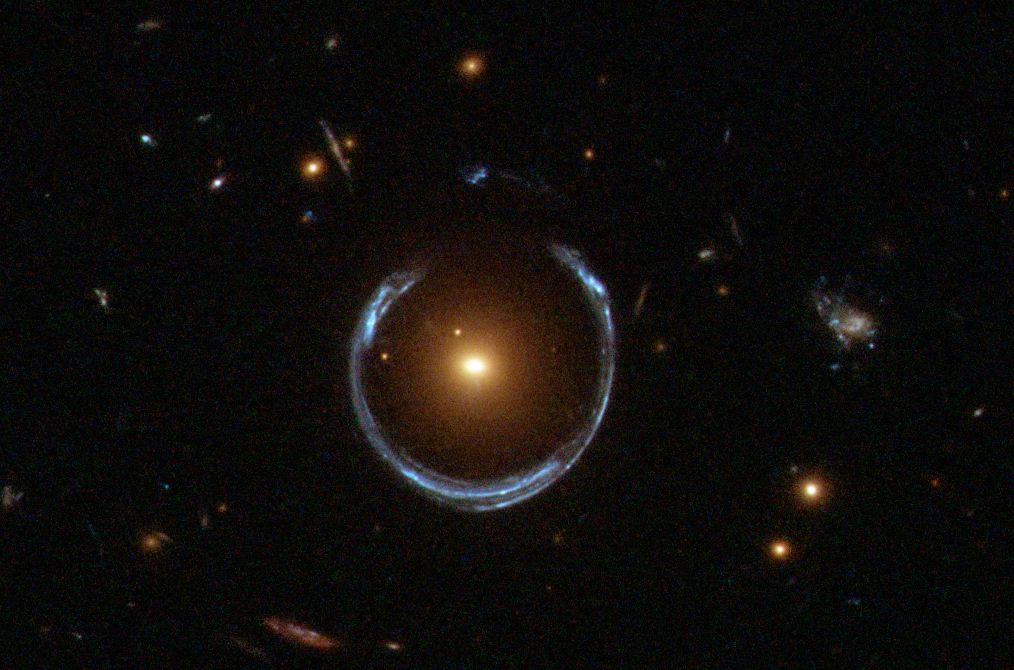
\includegraphics[scale=0.4]{Figures/DarkMatterEvidence/Einstein_Ring_from_Hubble.JPG}
    \caption{An example of a "Horseshoe Einstein Ring" created by the bending of light from a distant blue galaxy by the central red galaxy LRG 3-757 [ESA/Hubble]}
    \label{fig:DM_Evidence_Einstein_Ring}
\end{figure}

\par
Based on the amount of distortion, the mass of the object causing the lensing can be measured and can be applied to both individual galaxies as well as clusters.
The mass required for the lensing observed can then be compared to the luminous mass, which also shows a mismatch between the two \cite{History_Of_Dark_Matter_2018_ref}.


\par
At the galactic cluster scale there is the yet more evidence of the missing mass, which we'll now show for the galactic cluster 1E0657-558, also known as the Bullet Cluster.
This galaxy cluster was formed by the merger of two smaller clusters \cite{bullet_cluster_ref}.
In the resultant Bullet Cluster the baryonic matter can be tracked via electromagnetic radiation and the mass via lensing.
Observations show that there is a discrepancy between the centre of mass and the observed centre of mass, shown in \autoref{fig:DM_Evidence_Bullet_Cluster}.
The luminous matter from each of the smaller clusters mixed, causing the matter to slow down.
On the other hand, the majority of the mass has passed through.
What this indicates is that in addition to there being a significant invisible mass, this mass must also have a very small cross-section with baryonic matter and itself.

\begin{figure}[!htbp]%
    \centering
     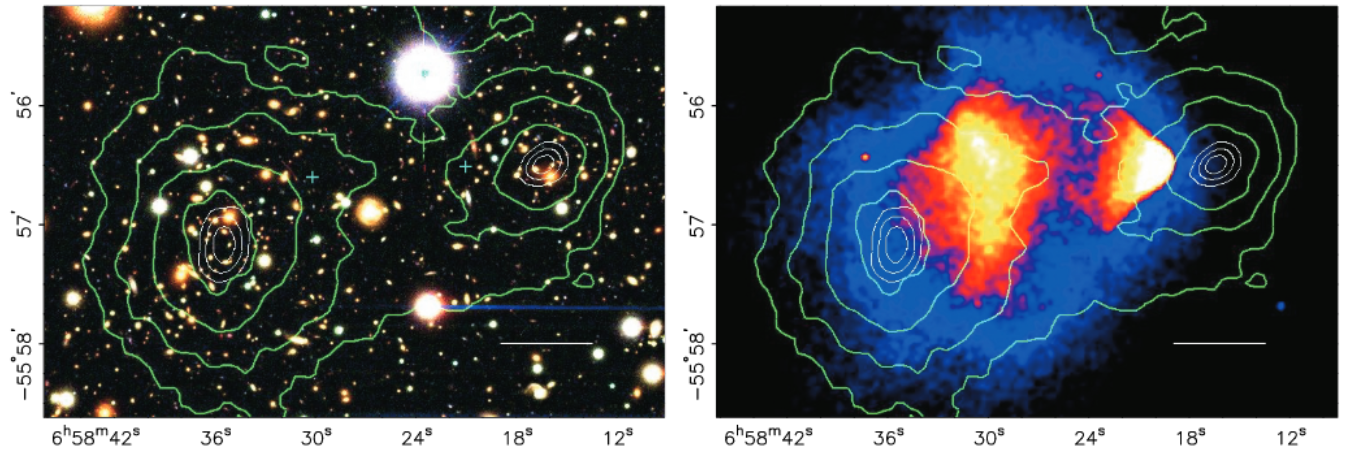
\includegraphics[width=\textwidth]{Figures/DarkMatterEvidence/bullet_cluster_2.png}
    \caption[Merging of two galaxy cluster, 1E 0657-558]{Merging of two galaxy clusters: The Bullet Cluster, 1E 0657-558.
             During the collision, the dark matter components passed through without interacting.
             The baryonic components from the two clusters interacted, causing them to lag behind .
             \textbf{Left:} Optical image from the Magellan observatory.
             \textbf{Right:} X-ray image from the Chandra observatory.
             In both figures the white bar indicates 200 kpc, the green contours are the mass distribution from weak-lensing reconstructions and the white contours are the errors on the position of the lensing peaks.
             Figure adapted from \cite{bullet_cluster_ref}.}
    \label{fig:DM_Evidence_Bullet_Cluster}
\end{figure}


\subsection{Cosmological Scale}
\par


\par
What is often quoted as the strongest evidence for dark matter comes from the cosmic microwave background (CMB) radiation which was first discovered in 1965 \cite{cmb_origins_ref}.
This is a near perfectly uniform field of microwave photons with the energy spectrum of a 2.7225 K blackbody, shown in \autoref{fig:DM_Evidence_CMB_Map}.
These photons, sometimes referred to as `relic' radiation, last interacted with with the early universe, when the temperature was almost 3000 K \cite{bigbang_nucleosynthesis_ref}.
This was some 380,000 years after the Big Bang\footnote{The surface of last scattering}, before the universe cooled sufficiently for recombination\footnote{When electrons were first able to bind to nuclei} and neutral Hydrogen formation.
At this time, the universe was filled with a plasma as there was enough energy to ionise an atom as soon as it has been formed.
The CMB photons decoupled from the plasma during this time and was able to were able to free-stream through the universe.
As the universe has expanded, these photons have red-shifted down to the now observed microwave photons, and give an insight into the early universe \footnote{It has also been quoted as ``a selfie of the baby universe" \cite{marisarthurs_thesis_ref}}.

\begin{figure}[!htbp]%
    \centering
    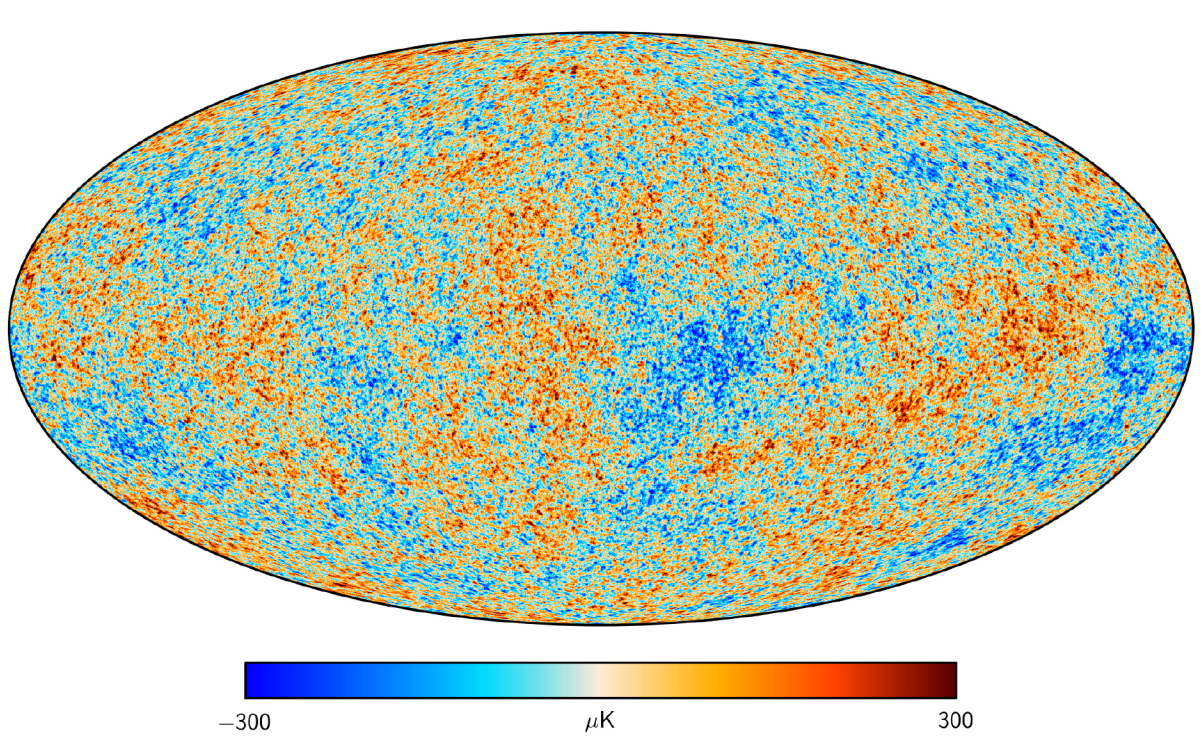
\includegraphics[width=0.8\textwidth]{Figures/DarkMatterEvidence/cmb_radiation.png}
    \caption[Temperature fluctuations of the CMB radiation]{Temperature fluctuations of the CMB radiation from Planck.
             The maximum difference between the warmest (red) and coldest (blue) is 0.0006K.
             Figure from \cite{plank_result_ref}.}
    \label{fig:DM_Evidence_CMB_Map}
\end{figure}

\par
At the time when the CMB decoupled the universe was extremely isotropic, which can be seen in the uniformity of the CMB, though there are minor anisotropies.
Prior to recombination, any small non-uniformity in the plasma resulted in a gravitation well, into which all forms of matter were pulled into.
The inward force of gravity competed with the outward force from photons, tied with the expanding (and therefore cooling) universe resulted in standing pressure waves in the plasma, referred to as baryon acoustic oscillations (BAO), and describe the temperature fluctuations.
Describing them as spherical harmonics ($Y_{lm}(\theta,\phi)$, the temperature fluctuations can be written as \cite{History_Of_Dark_Matter_2018_ref}:
\begin{equation}
    \frac{\delta T}{T}(\theta, \phi) = \sum_{l} \sum_{m} a_{lm}Y_{lm}(\theta,\phi)
    \label{eq:bao_spherical_harmonics}
\end{equation}
The temperature fluctuations between two points in the CMB can then be described by:
\begin{equation}
    C(\theta) = \frac{1}{4\pi} \sum_{l} (2l + 1) C_l P_l (cos(\theta))
\end{equation}
where $\theta$ is the angular separation between two points and $P_l (cos(\theta))$ are Legendre polynomials.
$C_l$ can be considered as the magnitude of the temperature fluctuation when $l$ is large, making $l$ analogous to $\theta$.
The application of this on the lasted Planck result is shown in \autoref{fig:DM_Evidence_BAO} \cite{plank_result_ref}.
\begin{figure}[!htbp]%
    \centering
    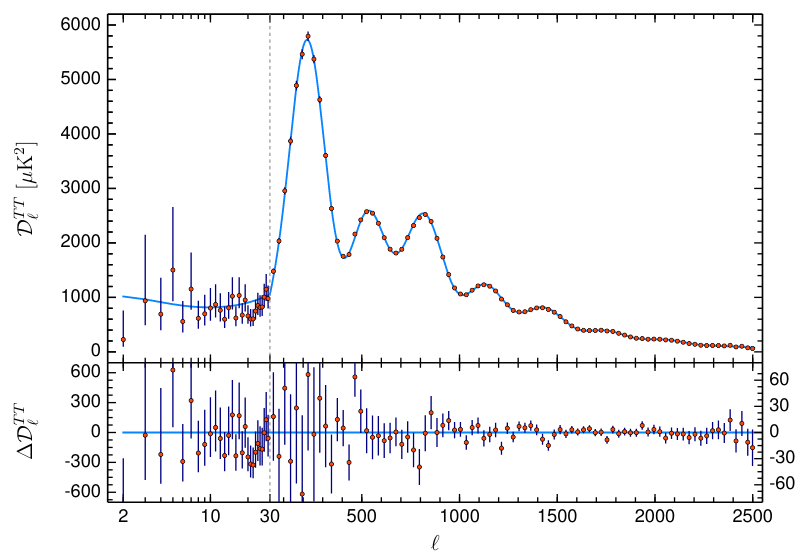
\includegraphics[width=0.8\textwidth]{Figures/DarkMatterEvidence/bao.png}
    \caption[Temperature fluctuations of the CMB spectrum as a function of $l$]{The temperature fluctuations of the CMB power spectrum against the spherical harmonics multipole parameter, $l$, which is a proxy for angular separation.
             \textbf{Top:} the power spectrum fitted to the $\Lambda$CDM model.
             \textbf{Bottom:} the residuals of the fit, shown to be small.
             Figure from \cite{plank_result_ref}.}
    \label{fig:DM_Evidence_BAO}
\end{figure}
\par
The shape of the spectrum in \autoref{fig:DM_Evidence_BAO} sets significant constraints on the $\lambda$CDM model, with the latest Planck result, the observed CMB is best fitted with a energy density in the universe divided up as: 4.88\%$\pm$0.03\% baryonic matter, 26.01\%$\pm$0.22\% and the remaining 69.11\%$\pm$0.62\% being dark matter \cite{plank_result_ref}.

\section{Candidates}
\par
With there being a plethora of evidence that "something is there", we can turn our attention to what it might be.
From the observation, we can say that an potential candidate for dark matter must be;
\begin{itemize}
    \item Weakly, or not interacting via electromagnetism 
    \item Weakly, or not interacting via the strong force
    \item Have some kind of clustering; either by being slow moving (cold) or some other way
    \item Not baryonic matter
    \item Stable over the timescale of the Universe.
\end{itemize}
Additionally, it may be beneficial to start with the Standard Model of particle physics, and look for extensions which satisfy the above requirements.
In this section a brief description of proposed candidates are described briefly, followed by possible the most favoured candidate; the weakly interacting massive particle (WIMP)
It should be noted that many of these particles.

\subsection{MACHOs and primordial black holes}
\par
The first set of candidates seems like a very good candidate on the surface.
Massive astrophysical compact halo objects (MACHOs) are objects such as star remnants, very faint stars and 
and primordial black holes are non-luminous.
These have been some of the earliest possible explanations and have been favourable as they don't require new matter.

\par
Microlening surveys are able to observe objects with XYZ properties, but are limited to XYZ masses.
If such 
Unfortunately microlening searching have shown that MACHOs cannot make up more than 25\% of galactic halo masses.

\par
Black holes are also a contributor. 
These are a favoured solution as well as they are comprised of understood matter, and will the LIGO collaboration having measuring the merger of black holes, and the first image of a black hole being taken in XXX, our understanding of them as a component is increasing.
However, black holes such as that at the centre of the Milky Way are not believed to have been around in the minutes after the Big Bang but rather from the collapsing of some of the earliest super massive stars.
Instead, primordial black holes must have existed, formed from a different process in the early minutes after the Big Bang.
This is supported by some of the measurements from LIGO such as the merger of black holes of around 30 solar masses.
A black hole of this mass is not as likely to be produced from the regular stellar evolution.
Assuming that there are indeed primordial black holes, then they would contribute at least in part to dark matter.
If these primordial black holes were to be the dominant explanation for dark matter, then the model for the formation of the early universe needs addressing.
Our understanding on this topic is still evolving and the amount that this contributes to dark matter will be pinned down.

\subsection{Modified Gravity}
\par

\subsection{Neutrinos}
\par
One of the first candidates suggested as dark matter were neutrinos: the stable, long-lived and weakly-interacting particles in the standard model.
Unfortunately, N-body simulations shown that given the relativistic velocities are inconsistent with the structural formations that we observe \cite{neutrinos_and_galaxy_clustering_ref}. 
This has not ruled out neutrinos entirely, with a new species suggested which interacts only gravitational \cite{sterile_neutrinos_ref}.
Postulated to have a small mixing angle with standard model neutrinos, this would allow for limited interaction between this dark matter and SM matter.
\par
The most recent excitement around this is an unidentified 3.55keV line in X-ray spectra from several galactic clusters with high dark matter content \cite{sterile_neutrino_xray_decay_ref}, with one possible interpretation is the decay of sterile neutrinos, though there is much debate around this \cite{xray_from_sterile_neutrons_2_ref, xray_from_sterile_neutrons_3_ref}.
Separately, results by MicroBooNE have indicated neutrino mixing that is inline with the standard model, going against previous results from MiniBooNE where an excess in neutrino oscillations \cite{miniboone_and_microboone_sterile_neutrino_ref}.
The BEST experiment has also pointed towards sterile neutrinos to account for the deficit observed in germanium isotope production \cite{best_sterile_neutrino_result_ref,best_sterile_neutrino_2_ref}.
With the correct properties, the sterile neutron could contribute to dark matter, though as the understanding of the neutrinos we already know about contains significant gaps (such as the mass hierarchy), more work is needed \cite{sterile_neutrino_as_dm_ref, sterile_neutrinos_dm_ref}.

\subsection{Axions}
\par
Hypothesised in 1977, axions were postulated to solve the strong CP problem of the standard model \cite{axion_origins_ref}.
Axions are a pseudo-Goldstone boson generated by spontaneous symmetry breaking at some energy scale, $f_a$, with the mass of this particle predicted to follow:
\begin{equation}
    m_a \approx (0.6eV)\frac{10^7 GeV}{f_a}
\end{equation}
The value of $f_a$ is constrained to be greater than that of the electroweak symmetry-breaking scale, given exciting constraints on experiments.
This leaves a particle with a mass between 10${}^{-6}$ and 10${}^{-2}$eV for which they could account for dark matter \cite{axions_ref}.
\par
There are multiple proposed production mechanisms for axions such as via thermal production in the early universe.
However, axions produced in this fashion would contribute to hot dark matter the constraints are very limitting \cite{hot_axions_ref}.
Separately, slower, non-relativistic axions can be created through other processes such as "re-alignment mechanism" \cite{cold_axion_ref}.
\par
Axions may couple to photons, allowing for a conversion to microwaves.
These can be searched for in a microwave cavity with a strong magnetic field applied to it.
In this situation it is expected that the axion will convert into monochromatic microwave photons.
The ADMX experiment has adopted this approach and is currently the most sensitive experiment to this \cite{admx_experiment_ref}.
\par
Another search of axions is where an axion is absorbed and an atomic electron is ejected.
This electron is then detectable as an electronic recoil.
These searches are typically performed by large underground direct dark matter experiments, with the tightest constraint on axio-electric coupling coming from XENONnT \cite{xenonnt_sr1_er_ref}.
\par
A third approach is via laser beams whereby a beam is propagated between two superconduction magnets that are optically separated.
If axions are coupling to photons, then the initial beam will transform into an axion and then later convert back, allowing the light to be seen through the optical barrier.
Though not as sensitive as the other axion-photon conversion approaches, it does not have the same uncertainties associated with astrophysics and cosmology.
Two notable experiments using this approach are ALPS \cite{alps_axion_result_ref} and OSQAR \cite{osqar_axion_result_ref}. 
\par
Other search methods are also being explored such as axion induced nuclear electric dipole moment (see CASPEr \cite{casper_experiment_ref}), axion to X-ray conversion in the presence of a magnetic field (see IAXO \cite{iaxo_experiment_ref}), and energy-loss in galactic observables such as supernova explosions due to axion-electron coupling \cite{axions_from_supernova_ref}.

\subsection{WIMPS}
\label{sec:wimp_as_a_candidate}
\par
Another candidate, are arguably the most popular is a set of new particles that interact via the weak force, but have a lot of mass.
Namely, Weakly Interacting Massive Particles (WIMPs)\footnote{this differs from the original meaning where the interaction probability was low}. 
\par
In this case, dark matter is formed of stable particles from the early universe.
At this time, WIMPs were in thermal equilibrium with the rest of the universe: so the self-annihilation rate was equal to that of the creation rate from interactions between light particles.
As the universe expanded, the density of WIMPs decreased until the self-annihilation rate dropped.
Referred to as "thermal freeze-out", the remaining WIMPs appear as a relic abundance. 




\par
Known as the "WIMP miracle", this connection between cosmology and particle physics has helped give WIMPs the prevalence it has.


\par
Additionally, there are certain extensions to the standard model which are able to solve problems including the hierarchy problem and gauge coupling unification which also produce a WIMP candidate.


\par
In addition to supyersymmetry, WIMP-like dark matter particles do appear from other theories.
The typical search strategy for WIMPs by large underground detectors such as LUX-ZEPLIN \cite{LZ_TechnicalDesignReview_ref}, XENONnT \cite{xenonnt_projected_sensitivty_ref} and PandaX-4T \cite{pandax_4t_ref}.
